\documentclass{amsart}
\usepackage{fullpage}

\usepackage[T1]{fontenc}
\usepackage[utf8]{inputenc} 
\usepackage{lmodern}
\usepackage[slovene]{babel}
\usepackage{hyperref}
\usepackage{amsmath,amssymb,amsfonts, mathtools}
\usepackage{bbm}
\usepackage{graphicx}
\graphicspath{{./images/}}

\linespread{1.2}

\newcommand{\N}{\mathbb{N}}
\newcommand{\Z}{\mathbb{Z}}
\newcommand{\Q}{\mathbb{Q}}
\newcommand{\R}{\mathbb{R}}
\newcommand{\C}{\mathbb{C}}

% ukazi za matematicna okolja
\theoremstyle{definition} % tekst napisan pokoncno
\newtheorem{definicija}{Definicija}[section]
\newtheorem{primer}[definicija]{Primer}
\newtheorem{opomba}[definicija]{Opomba}

\renewcommand\endprimer{\hfill$\diamondsuit$}


\theoremstyle{plain} % tekst napisan posevno
\newtheorem{lema}[definicija]{Lema}
\newtheorem{izrek}[definicija]{Izrek}
\newtheorem{trditev}[definicija]{Trditev}
\newtheorem{posledica}[definicija]{Posledica}

\title{Kontekstno-neodvisne gramatike za kodiranje in stiskanje podatkov}
\author{Janez Podlogar}
\date{\today}

\begin{document}

\begin{abstract}

    V delu predstavimo motivacijo in definicije, ki so potrebni za obravnavnje
    stiskanja podatkov s kontekstno-neodvisnimi gramatikami.

\end{abstract}

\maketitle

\section{Kodiranje podatkov}

Zapis informacije v neki obliki ni primeren za vsakršno rabo. Besedilo, zapisano z 
pismenkami, je neberljivo za slepe osebe, saj je komunikacijski kanal v tem primeru
vid. Prav tako pisanega besedila v pravotni obliki ni moč poslati z telegrafom. V tem
primeru je komunikacijski kanal žica in pismenke se po njej ne morejo sprehoditi. V obeh 
primerih je informacija, ki bi jo radi prenesli v neprimerni obliki. V prvem 
primeru je potrebno besedilo zapisati z Braillovo pisavo. V drugem primeru pa je 
potrebno besedil pretvoriti v električni signal. Spreminjanje zapisa sporočila
pravimo \textit{kodiranje}, sistemu pravil, po katerem se kodiranje opravi,
pa \textit{kod}. 

\begin{primer}\label{Morse}

    \textit{Morsejeva abeceda} je kodiranje črk, števil in ločil s pomočjo zaporedja kratkih
    in dolgih signalov:

    \begin{itemize}
        \item Dolžina kratkega signala je ena enota.
        \item Dolgi signal je trikrat daljši od kratkega signala.
        \item Razmiki med signali znotraj znaka so dolžine kratkega signala.
        \item Presledki med znaki so dolgi tri kratke signale oz. en dolgi signal.
        \item Presledki med besedami so dolgi sedem kratkih signalov.
    \end{itemize}

    \begin{figure}[h]
        \centering
        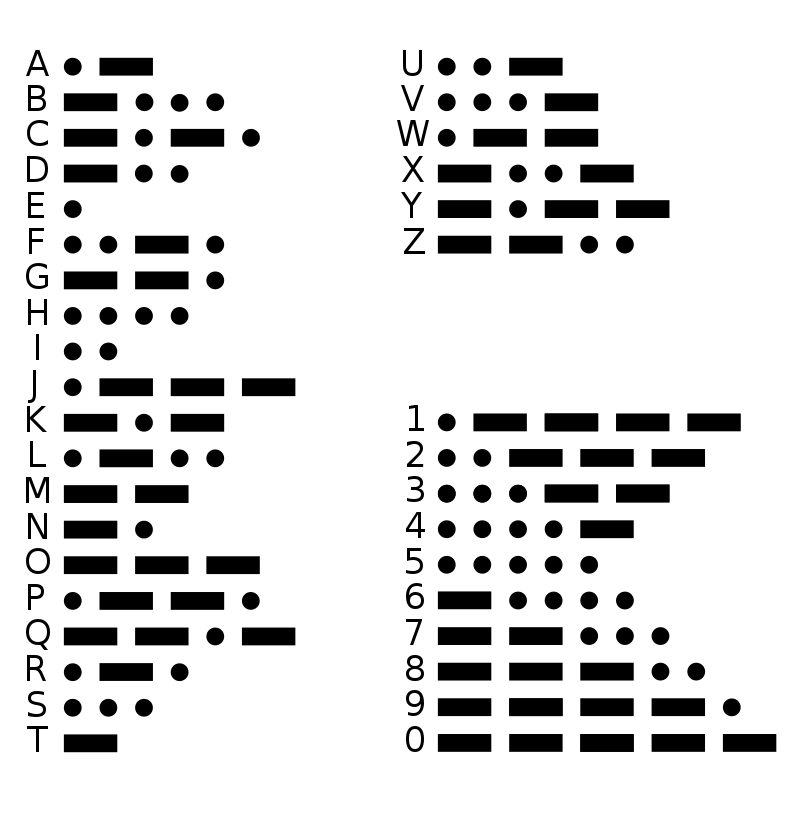
\includegraphics[width=4.3cm]{International_Morse_Code.svg.png}
        \caption{Mednarodna Morsejeva abeceda}
        \label{fig:Morse}
    \end{figure}

    Prvotni namen Morsejeve abecede je komunikacija preko telegrama, saj komunikacijski
    kanal dovoljuje le električne signale in tišino med njimi. Kodiranje črk je takšno,
    da imajo črke z višjo frekvenco (v angleškem jeziku) krajši zapis, s tem se dolžina
    kodiranega sporočila skrajša in posledično tudi čas prenosa.

\end{primer}

\begin{definicija}

    \textit{Abeceda} je končna neprazna množica $ \Sigma $. Elementom abecede pravimo \textit{črke}.
    \textit{Množica vseh končnih nizov abecede} $ \Sigma $ je

    \[
        \Sigma^* = \{ a_1 a_2 a_3 \cdots a_n \mid n \in \N_0 \land \forall i: a_i \in \Sigma \}, 
    \]
    kjer za $ n = 0 $ dobimo prazen niz, ki jo označimo z $ \varepsilon $.
    \textit{Dolžino niza w} označimo z $ |w| $ in je enaka številu črk v nizu $ w \in \Sigma^* $.
    \textit{Jezik na abecedi} $ \Sigma $ je poljubna podmnožica množice $ \Sigma^* $. 

\end{definicija}

\begin{opomba}
    
    \textit{Kleenejeva zvezdica} ali \textit{Kleenejevo zaprtje} je operacija, ki
    abecedi $ \Sigma $ priredi najmanjšo nadmnožico $ \Sigma^* $, ki vsebuje
    \textit{prazen niz} $ \varepsilon $ in je zaprta za konkatenacijo oziroma veriženje.
    Z drugimi besedami, $ \Sigma^* $ je množica vseh končnih nizov, ki
    jih lahko generiramo z veriženjem črk abecede $ \Sigma $. \\
    Za abecedo $ \Sigma $ definirajmo
    \begin{align*}
        & \Sigma^0 = \{ \varepsilon \} \\
        & \Sigma^1 = \Sigma \\
    \end{align*}
    ter za vsak $ i > 0 $ rekurzivno
    \[
        \Sigma^{i+1} = \{ wa \mid w \in \Sigma^i \text{ in } a \in \Sigma \},
    \]
    potem je Kleenejeva zvezdico na $ \Sigma $ enaka
    \[
        \Sigma^* = \bigcup_{i \geq 0} \Sigma^i
    \]

\end{opomba}



\begin{primer}
    
    Naj bo $ \Sigma = \{ a,b,c \} $ abeceda, potem je
    \begin{gather*} 
        ab \in \Sigma^* \\
        ccc \in \Sigma^* \\
        cababcccababcccab \in \Sigma^*
    \end{gather*}

\end{primer}

\begin{definicija}
    
    \textit{Kodiranje nizov abecede} $ \Sigma $ je obrnljiva funkcija $ K \colon \Sigma^* \to \Sigma_c^* $,
    kjer je $ \Sigma_c $ \textit{kodirna abeceda}. $ K(w) $ imenujemo \textit{koda niza} $ w $.
    \textit{Dekodiranje} je obraten postopek, ki za podano kodo $ c \in \Sigma_c^* $ vrne prvoten niz
    $ w \in \Sigma^* $, ki smo ga kodirali.

\end{definicija}

\begin{primer}
    
    Formalizirajmo Morsejevo abecedo iz Primera~\refeq{Morse}. Abecedi sta
    \begin{gather*}
        \Sigma = \{ \text{A},  \text{B}, \ldots, \text{Z} \} \, \cup \, \{ 0, 1, \ldots, 9 \} \, \cup \, \{ \_ \} \\
        \Sigma_c = \{ ., -, \_, \_\_\_ \} \\
    \end{gather*}
    Definirajmo kodno funkcijo črk abecede $ \kappa \colon \Sigma \to \Sigma_c^* $, ki vsakei črki iz abecede
    priredi niz črk kodirne abecede. Funkcija je definirana s tabelo iz Slike~\refeq{fig:Morse},
    dodatno $ \kappa(\_) = \_\_\_ $ . Za niz $ w = a_1a_2 \ldots a_n \in \Sigma^* $ definiramo kodirno 
    funkcijo $ K $ po črkah
    \[
        K(w) = \kappa(a_1)\kappa(a_2)\cdots\kappa(a_n)
    \]
    Opazimo, da je Morsejeva abeceda kodiranja brez izgube.

\end{primer}

\section{Stiskanje podatkov}

Eden izmed namen kodiranja je tudi doseči čim večjo ekonomičnost zapisa. Želimo, da bi bilo naše sporočilo
čim krajše. Kodiranje, ki skrajša zapis podatkov, imenujemo \textit{stiskanje podatkov}.

\begin{definicija}
    
    \textit{Stiskanje} je kodiranje $ K $ za katerega velja 
    \[ 
    \forall w \in \Sigma^* \colon \left\lvert K(w)\right\rvert \ll \left\lvert w \right\rvert
    \]

\end{definicija}

% \begin{opomba}
    
%     Za \textit{kodiranje brez izgube} velja
%     \[
%         \forall w \in \Sigma^*: K^{-1}(K(w)) = w
%     \]
%     Za \textit{kodiranje z izgubo} velja
%     \[
%         \exists w \in \Sigma^*: K^{-1}(K(w)) \approx w
%     \]

% \end{opomba}

\begin{primer}\label{Kompresija}
    
    Za abecedo vzemimo $ \Sigma = \{ a,b,c \} $ in poglejmo niz
    \[
        w = cababcccababcccab
    \]
    Opazimo, da se nam v nizu $ w $ večkrat ponovita vzorca $ ab $ in $ ccc $. Zato
    uvedemo novi spremenljivki $ A_1 = ab $ in $ A_2 = ccc $. Sedaj lahko zapišemo $ w $ kot
    \[
        w = cA_1A_1A_2A_1A_1A_2A_1
    \]
    Ponovno se nam pojavi vzorec, tokrat $ A_1A_1A_2 $. Uvedemo novo spremeljivko $ A_3 = A_1A_1A_2 $
    in zapišemo $ w $ kot
    \[
        w = cA_3A_3A_1
    \]
    Prvotni niz smo z novimi spremeljivkami skrajšali. Kot bomo videli, smo
    pretvorili niz $ w $ v kontekstno neodvisno gramatiko $ G_w $ s
    produkcijskimi pravili
    \begin{align*}
        & A_0  \rightarrow  cA_3A_3A_1, \\
        & A_1  \rightarrow  ab, \\
        & A_2  \rightarrow  ccc, \\
        & A_3  \rightarrow  A_1A_1A_2
    \end{align*}

\end{primer}

\section{Kontekstno-neodvisne gramatike}

\begin{definicija}

    \textit{Formalna gramatika} $ G $ so pravila, ki nam iz abecede $ \Sigma $ tvorijo jezik
    $ L(G) $

\end{definicija}

\begin{definicija}

    \textit{Kontektsno-neodvisna gramatika} je četverica $ G = ( V, \Sigma, P, S ) $, kjer je
    $ V $ končna množica \textit{spremenljivk}, abeceda $ \Sigma $ množica \textit{končnih simbolov} tako,
    da $ \Sigma \cap V = \emptyset $, $ P \subseteq V \times ( V \cup \Sigma )^* $ relacija, ki ji
    pravimo \textit{produkcijsko pravio} in $ S \in V $ \textit{začetna spremenljivka}.

\end{definicija}

\begin{definicija}
    
    Naj bo $ G = ( V, \Sigma, P, S ) $ kontekstno-neodvisna gramatika. Naj bodo $ \alpha $,
    $ \beta $, $ \gamma \in ( V \cup \Sigma )^* $ nizi spremenljivk in končnih simbolov,
    $ A \in V $ spremenljivka ter naj bo $ ( A, \beta ) \in P $ produkcijsko pravilo,
    označimo ga z $ A \rightarrow \beta $. Pravimo, da se $ \alpha A \gamma $ 
    \textit{prepiše s pravilom} $ A $ v $ \alpha\beta\gamma $, pišemo $ \alpha A \gamma  \Rightarrow 
    \alpha\beta\gamma $. Pravimo, da $ \alpha $ \textit{porodi} $ \beta $, če je $ \alpha = \beta $ ali če
    za $ k \geq 0 $ obstaja zaporedje $ \alpha_1, \alpha_2, \ldots \alpha_n
    \in ( V \cup \Sigma )^* $ tako, da 
    \[
        \alpha \Rightarrow \alpha_1 \Rightarrow \alpha_2 \Rightarrow \ldots \Rightarrow \alpha_n
        \Rightarrow \beta
    \]
    in pišemo $ \alpha \xRightarrow{*} \beta $.

\end{definicija}

\begin{posledica}

    Jezik kontekstno neodvisne gramatike $ G $ je
    \[
        L(G) = \{ w \in \Sigma^* \mid S \xRightarrow{*} w \}
    \]

\end{posledica}

\begin{opomba}
    
    Ime kontekstno-neodvisna gramatika izvira iz oblike produkcijskih pravil. Na levi
    strani produkcijskega pravila mora vedno stati samo spremenljika. Torej vsebuje samo
    pravila oblike
    \[
        A \rightarrow \alpha,
    \]
    kjer je  $ A \in V $ in $ \alpha \in ( V \cup \Sigma )^* $. Ne sme pa vsebovati
    pravila oblike
    \[
        \alpha A \gamma \rightarrow \alpha\beta\gamma,
    \]
    kjer je $ A \in V $ in so $ \alpha, \beta, \gamma \in ( V \cup \Sigma )^* $, saj je
    pravilo odvisno od predhodnega konteksta. Odvisno je od tega ali pred njim stoji $ \alpha $
    in za njim $ \beta $.

\end{opomba}

\begin{primer}
    
    Formalizirajmo gramatiko iz Primera~\refeq{Kompresija}, ki smo jo generirali z nizom
    $ w = cababcccababcccab $. Označimo jo z $ G_w = ( V, \Sigma, P, S ) $, kjer je 

    \begin{gather*}
         V = \{ A_0, A_1, A_2, A_3 \}, \\
         \Sigma = \{ a, b, c \}, \\
         P = \{ A_0  \rightarrow  cA_3A_3A_1, A_1  \rightarrow  ab, A_2  
        \rightarrow  ccc, A_3  \rightarrow  A_1A_1A_2 \}, \\
         S = A_0
    \end{gather*}
    Vidimo, da $ G_w $ ustreza naši definiciji kontekstno-neodvisne gramatike
    in res kodira $ w $, saj je 
    \[
        L(G_w) = \{w\}
    \]

\end{primer}



\[
    x \rightarrow G_x \rightarrow B(G_x)
\]

\end{document} 